\chapter{Digital filter design}
	
	In general \de{filters} are realised/implemented in the discrete-time case because, in opposition to the continuous-time one, they are easier to implement (they are in fact algorithm).
	
	Given a linear time-invariant discrete-time causal system with impulse response $h(n)$, it's output to a sinusoidal input in the form $x(n) = A e^{j(\omega_0n + \phi_0)}$ is determined by the convolution $x(n)*h(n)$ and by expanding the definition we can see that
	\begin{align*}
		y(n) & = \sum_{k=0}^\infty A e^{j(\omega_0(n-k)+\phi_0)} h(k) = A e^{j\phi_0} e^{j\omega_0n} \sum_{k = 0}^\infty h(k) e^{j\omega_0k} \\
		& = A e^{j(\omega_0n+\phi_0)} H(e^{j\omega_0})
	\end{align*}
	We can indeed see that the output of the system is still a sinusoidal function with unchanged frequency $\omega_0$ but with phase and magnitude \textit{re-scaled} the transfer function $H$ evaluated at the point $e^{j\omega_0}$ in the frequency domain. In particular the term $H(e^{j\omega_0})$ is the eigenvalue associated to the eigenfunction $e^{jn\omega_0}$; getting rid out of the complex notation the output can also be rewritten as
	\[ y(n) = A \big| H(e^{j\omega_0}) \big| \cos\Big( \omega_0 n + \phi_0 +\angle H(e^{j\omega_0}) \Big) \]
	where $|H(e^{j\omega_0})|$ is the \textbf{gain} of the system and $\angle H(e^{j\omega_0})$ is it's \textbf{phase shift} (a sort of \textit{delay}) evaluated for the frequency $\omega_0$.
	
	\begin{SCfigure}[2][bht]
		\centering 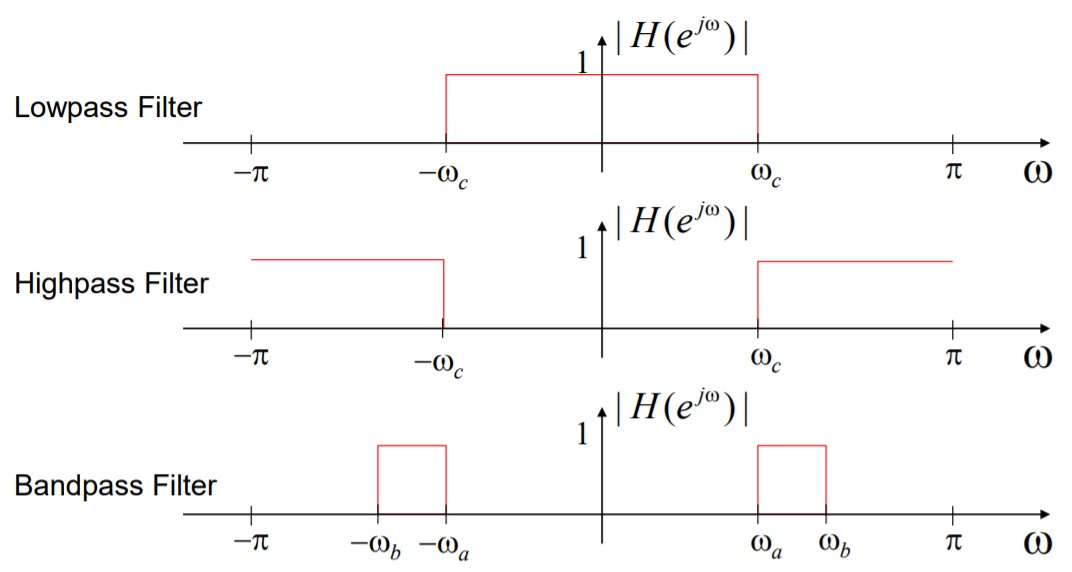
\includegraphics[width=8cm]{ideal-filters}
		\caption{examples of ideal filters in the frequency domain.}
		\label{fig:filt:idealfilter}
	\end{SCfigure}
	
	In figure \ref{fig:filt:idealfilter} a list of \textbf{ideal filters} are presented in the frequency domain, however they are not feasible: they are in fact \textbf{non-causal} system (it means that to create them we should have $h(n)\neq 0$ for $n<0$), meaning that in order to apply their definition we have to count on an infinite set of samples (which isn't possible to compute).
	
	\paragraph{Low pass filter} A low pass filter (or any generic filter) can be practically implemented by constructing a proper window function $w(n)$ that tends to \textit{simulate} the spectral behaviour of the ideal counter-part. Due to the fact that they are computed on a finite number of samples $M$, they originate a distorted frequency response (respect to the ideal case) involving ripples and not infinite slope on the cut-off frequency (as shown in figure \ref{fig:filt:windowfilter}).
	
	\begin{SCfigure}[2][bht]
		\centering 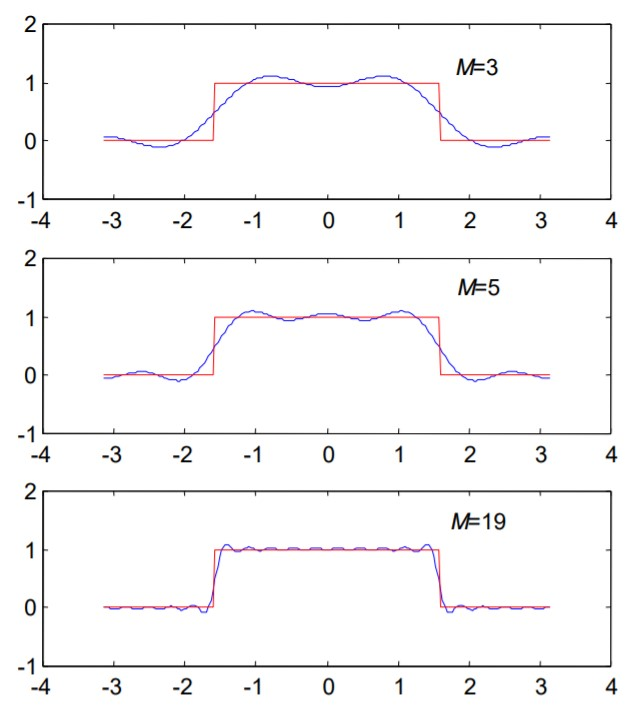
\includegraphics[width=5.5cm]{lpf-wind}
		\caption{spectral behaviour of low pass filter realised by appropriate windows of length $M$.}
		\label{fig:filt:windowfilter}
	\end{SCfigure}
	
	This ripples affect both the pass and stop band response due to the oscillations: the pass band gain is not constant and the stop band isn't univocally null.
	
\section{Filters specification}
	In general the realization of every digital filter is re-conducted on the design of a continuous-time low pass filter. Acknowledged that an ideal implementation isn't feasible in real world application, it's mandatory to define the following \textbf{design parameter} (assuming that the pass band gain is unitary):
	\begin{itemize}
		\item the maximum deviation $\delta_1$ from the pass-band gain; in particular the realised filter must be bounded in the range $[1-\delta_1,1]$;
		\item the maximum deviation $\delta_2$ from the 0 in the stop band region, and so it means that the gain in that zone must be inside the set $[0,\delta_2]$;
		\item the transition bandwidth defined as the difference of the minimum stop band frequency $\omega_s$ and the maximum pass band frequency $\omega_p$. 
	\end{itemize}
	The complete set of \textbf{specification parameters} $(\delta_1,\delta_2,\omega_p,\omega_s)$ can be synthesized in the \de{mask zone}, a graphical representation (figure \ref{fig:filt:mask}) in the frequency domain that represent the \textit{untouchable zones} by the filter and so determining the region on which the filter frequency response must behave.
	
	\begin{SCfigure}[2][bht]
		\centering 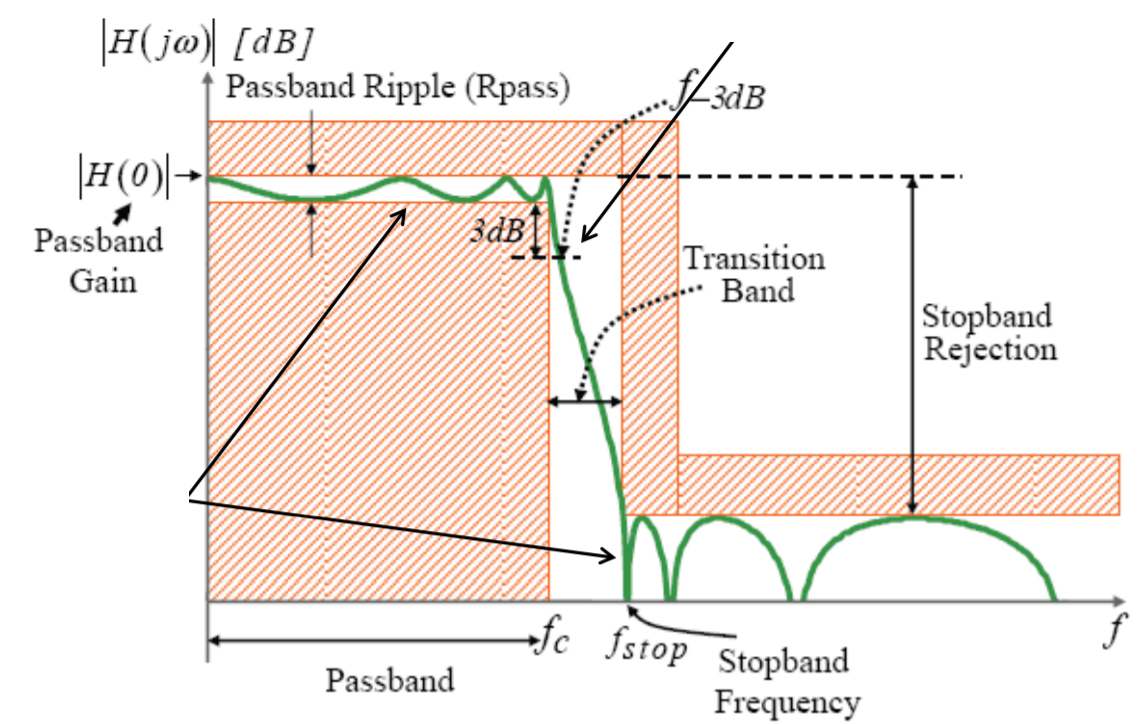
\includegraphics[width=7cm]{mask-zone}
		\caption{mask created to design a low pass filter.}
		\label{fig:filt:mask}
	\end{SCfigure}
	
	\paragraph{Phase distortion and group delay} Given a filter with impulse response $h(n)$, the phase shift of pure sinusoidal input function will be different depending on their frequency; in general in fact it happens that
	\[ \angle H(e^{j\omega_1}) \neq \angle H(e^{j\omega_2}) \qquad \qquad \textrm{with } \omega_1 \neq \omega_2 \]
	In particular application phase distortion is relevant and should be minimized, making it constant through-out all the pass-band region. As generalized concept we want a \de{group delay} defined as
	\begin{equation}
		\tau_g = -\frac{d\angle H(e^{(j\omega)}}{d\omega}
	\end{equation}
	that's ideally constant (as example with a value $\beta$) in the pass band. By integration we determine the desired linear phase shift equation $\angle H(e^{j\omega}) = - \beta \omega$, however the \textbf{generalized group delay} also consider an off-set phase distortion, determining the expression $\angle H(e^{j\omega}) = -\beta \omega + \alpha$.
	
	\paragraph{Design techniques} Depending on the type of filter wanted, completely different approach can be used:
	\begin{itemize}
		\item to realize infinite impulse response (IIR) filters it can be used the approximation of standard analog filter; the main drawback of this filters is that no-one of them present a linear phase response;
		
		\item to realize a finite impulse response (FIR) filters two methods can be used: one involving particular window functions and an algorithmic approach based on optimization techniques.
	\end{itemize}

\section{IIR filter design} \label{sec:filt:IIR}

	The design of any discrete-time infinite impulse response is based on the design of well established low-pass \textbf{prototypes} (that will be described) by generally following this stages:
	\begin{enumerate}
		\item convert the discrete-time filter specifications $\omega_p,\omega_s$ into the dual analogue $\Omega_p,\Omega_s$ for the continuous-time low-pass prototype;
		\item design the analog prototype considering some base reference(such the Butterworth, Chebyshev I and II, elliptic filters);
		\item return to the discretized domain using the impulse invariance (not object of study) or the bilinear transform methods.		
	\end{enumerate}
	This steps are used to develop a low-pass filter, however to design a more generic version two extra steps must be performed: the step 0 involving the transformation of the specification of the filter into a single low-pass  filter (in general transforming the frequency axis) and a fourth step that modify the computed on step 3 low-pass filter to determine the desired filter.
	
	\paragraph{Butterworth filter} The \textbf{Butterworth filter} is one of the simplest filter and uses the maximum deflect principle considering that the gain in the pass-band is unitary and all the derivative up to the order $N$ (that's also the \textbf{order} of the filter) are all zeros.
	
	The expression of the module of the filter is
	\begin{equation} \label{eq:filt:magbutter}
		\big|H_c(\Omega)\big|^2 = \frac{1}{1 + \left( \frac{\Omega}{\Omega_c} \right)^{2N}}
	\end{equation}
	where $\Omega_c$ is the \textbf{cut-off frequency} of the analog filter. As seen in figure \ref{fig:filt:buttanalog} the frequency response is strictly monotonically decreasing and, by increasing the order $N$ of the filter, also the \textbf{selectivity} (\textit{how narrow the transition bandwidth is}) increases.
	
	\begin{SCfigure}[2][bht]
		\centering 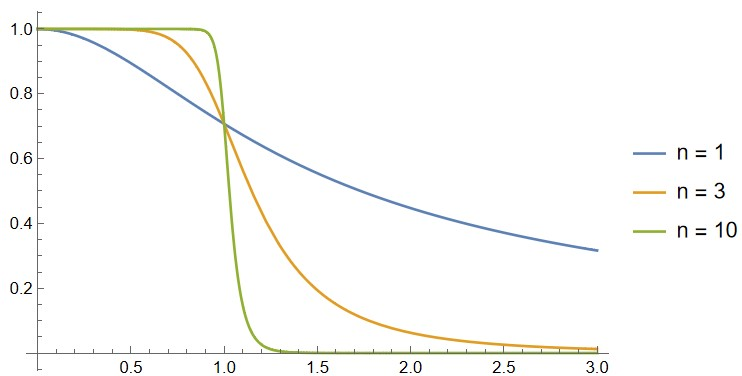
\includegraphics[width=8cm]{butter-time}
		\caption{frequency response of the Butterworth filter with cut-off frequency $\Omega_c=0$ for various order $N$.} \label{fig:filt:buttanalog}
	\end{SCfigure}

	The main drawback of this kind of implementation is that the phase distortion is strictly non-linear, however this effect can be neglected if far from the cut-off frequency (\ref{fig:filt:buttbode}).
	
	\begin{SCfigure}[2][bht]
		\centering 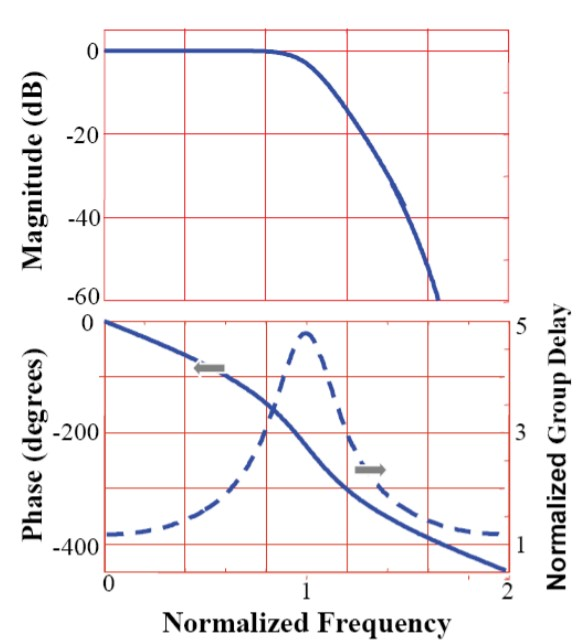
\includegraphics[width=5cm]{butter-bode}
		\caption{Bode plots of the response of the Butterworth filter.} \label{fig:filt:buttbode}
	\end{SCfigure}

	Considering the expression \ref{eq:filt:magbutter} it's possible to define the full complex expression of the filter considering that $|H_c(\Omega)|^2$ can be computed as
	\[ |H_c(\Omega)|^2 = H_c(s)\Big|_{s=j\Omega} H_c(-s)\Big|_{s=j\Omega} = \frac{1}{j\Omega + \left( -\frac {s}{\Omega_c} \right)^{2N} }\]
	This transfer function present no zeros (the roots of the numerator) but $2N$ poles that lies on the unit circle on the complex plane of the variable $s$; discharging the \textit{unstable points} for the poles it means that the roots presents phases of
	\[ \textrm{root's phases:} \qquad \frac \pi 2 + \big(2k+1\big) \frac{\pi}{2N}  \]
	
	
	\paragraph{Chebyshev type I} The \textbf{Chebyshev filter} of type I present a more complex expression respect to the Butterworth that's
	\begin{equation}
		\big|H_c(\Omega)\big|^2 = \frac 1 { 1 + \varepsilon^ 2 P_N^2 \big(\Omega/\Omega_c\big) }
	\end{equation}
	where $\varepsilon$ is the maximum ripple amplitude factor and $P_N(x)$ is the Chebyshev polynomial of order $N$ defined as $\cos (N\arccos x)$. Expanding the definition is possible to note that
	\[ P_0(x) = 1 \qquad P_1(x) = x \qquad P_2(x) = 2x^2-1 \qquad P_3(x) = 4x^3-3x \]
	and so the following recursive declaration of the polynomial can be stated: $P_N(x) = 2x P_{N-1}(x) - P_{N-2}(x)$. As shown in figure \ref{fig:filt:cheby-1bode}, this filter presents an equi-ripple behaviour in the pass-band (with ripples of values $\varepsilon$) that lead to a severe phase distortion in the same region, but it also presents a sharper transition bandwidth respect to the Butterworth filter.
	
	\begin{SCfigure}[2][bht]
		\centering 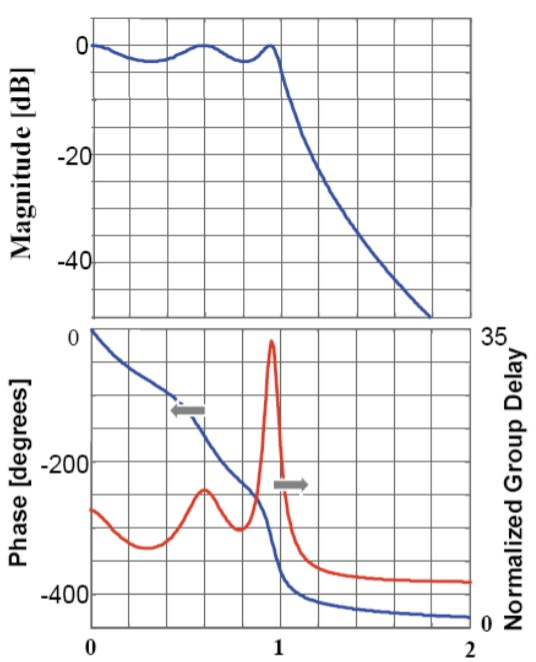
\includegraphics[width=5cm]{cheby-1}
		\caption{Bode plots of the response of the Chebyshev type I filter.} \label{fig:filt:cheby-1bode}
	\end{SCfigure}
	
	By doing a full analyses it's possible to state that that the poles of the transfer function lies on an ellipse in the complex plane with major diameter belonging to the imaginary axis and having value of $2$ (ranging from $-j$ to $j$); in particular the definition of the $k$-th pole (for a total of $N$ poles) is
	\[ s_k = r_1 \cos\phi_k + jr_2 \sin\phi_k  \]
	where $r_1 = \frac 1 2 \left( \alpha^{1/N} - \alpha^{-1/N} \right)$, $r_2 = \frac 1 2 \left( \alpha^{1/N} + \alpha^{-1/N} \right)$,  $\alpha = \frac 1 \varepsilon + \sqrt{1 + \frac 1 {\varepsilon^2}}$ and $\phi_k = \frac \pi 2 + (2k+1)\frac{\pi}{2N}$.
	
	\paragraph{Chebyshev type II and elliptic} The \textbf{Chebyshev} filter of type II is the dual representation of the first type one and presents and equi-ripple behaviour on the stop-band (with consequent phase distortion); the formal definition of the transfer function is the following:
	\begin{equation}
		\big|H_c(\Omega)\big|^2 = \frac 1 { 1 + \left[ \varepsilon^ 2 P_N^2 \big(\Omega/\Omega_c\big) \right]^{-1} }
	\end{equation}	
	This kind of filter is as selective as the previous one and presents poles that lies on an ellipse with major diameter belonging to the real part axis in the complex plane (and not the imaginary one).
	
	The \textbf{elliptic filter} is instead described by the Jacobian elliptic $U_N$ function determining the following transfer function
	\begin{equation}
		\big|H_c(\Omega)\big| = \frac{1}{1 + \varepsilon^2 U_N^2(\Omega/\Omega_c) }
	\end{equation}
	This filter presents an higher number of degrees of freedom (tweaking parameters of the Jacobian function $U_N$) leading to an higher selectivity (for a given value of $N$) respect to the previously described filters. This filter presents an equi-ripple behaviour both in the pass and stop-band.
	
	\paragraph{Comparison} Given a certain selectivity, the minimum required order $N$ for the filter changes and in fact it can be observed that
	\[ N_\textrm{elliptic} < N_\textrm{Chebyshev} < N_\textrm{Butterworth} \]
	Following this schema, going from left to right the computational complexity increases but also the expressions for the final design also becomes simpler to read.
	
\subsection{Finite difference methods}
	In the Laplace domain it can be observed that the complex variable $s$ corresponds to a differentiation in time of the transfer function, and so $\frac 1 s$ can be used for integration:
	\[ y(t) = \int_{-\infty}^t x(u)\, du \qquad \qquad \Rightarrow \qquad Y(s) = \frac 1 s X(s) \] 
	The same idea can be applied for discrete-time systems computing integrals with approximated equations; considering in fact the trapezoidal rule it can be shown that
	\[ \frac{y(n) + y(n-1)}{2} = \frac{x(n) - x(n-1)}{T} \qquad \xrightarrow{\Z} \quad \frac{Y(z) + z^{-1}Y(z)}{2} = \frac{X(z)-z^{-1} X(z)}{T}  \]
	\begin{equation} \label{eq:filt:bilinear}
		\frac{Y(z)}{X(z)} = \frac 2 T \frac{1 - z^{-1}}{1 + z^{-1} } = s
	\end{equation}
	Expression \ref{eq:filt:bilinear} refers to the \de{bilinear} (or Tustin) \de{differentiation} and can be used as rule to transform a transfer function in the $\Z$ complex plane (where discrete-time filters are described) to the $\mathscr L$ complex plane (used for continuous-time filters). With this idea stated we can say that the discrete-time $H(z)$ analogous of a continuous low-pass filter $H_c(s)$ can be computed as
	\begin{equation} \label{eq:filt:bilineartransfer}
		H(z) = H_c(s) \Big|_{s = \frac 2 T \frac{1 - z^{-1}}{1 + z^{-1} }}
	\end{equation}

	Inverting equation \ref{eq:filt:bilinear} it's possible to compute the transformation from the Laplace domain to the $\Z$ complex plane as
	\begin{equation}
		z = \frac{1 + \frac T2 s}{1 - \frac T2 s} \quad \xrightarrow{s = \sigma + j \Omega} \quad \frac{ 1 + \frac T 2 \sigma + j \frac T 2 \Omega}{1 - \frac T 2 \sigma - j \frac T 2 \Omega }
	\end{equation}
	
	\paragraph{Properties} It can be observed that the bilinear differentiation always preserves the system stability through discretization, in fact points lying in the half-plane with negative real part in the Laplace domain (region where the poles are stable for continuous-time systems) maps to the inner unit circle in the $\Z$ domain (where poles of discrete-time transfer function are stable). In particular it can be shown that the imaginary axis in the $s$ plane maps to the unit circle of the $z$ plane.
	
	\paragraph{Frequency warping} Considering pure imaginary variables in the Laplace domain (and so $s=j\Omega$) it can be observed from equation \ref{eq:filt:bilinear} that
	\[ j\Omega = \frac 2T \frac {1 - e^{-j\omega}}{1+ e^{-j\omega}} = j \frac 2 T \frac{e^{j\frac \omega 2} - e^{-j \frac \omega 2}}{e^{j\frac \omega 2 } + e^{-j\frac \omega 2 } } = j \frac 2  T \tan\left(\frac \omega 2 \right) \]
	It can so be seen that there's a sort of \textit{frequency warping} passing from the Laplace domain (continuous-time systems) and the $\Z$ domain one (that describes discrete-time systems):
	\begin{equation} \label{eq:filt:warping}
		\Omega  = \frac 2 T \tan\left( \frac \omega 2 \right) \qquad \qquad \qquad \omega = 2 \arctan\left(\frac{\Omega T}{2}\right)
	\end{equation}
	With this expression stated it can be observed that for $\Omega\rightarrow \infty$, the discrete-time frequency $\omega$ tends to the value $\pi$, resulting in a \textit{compression} of the spectrum and considering also that the expression are invertible it also means that no aliasing occurs as consequence of discretization.
	
\subsection*{Design steps}
	As previously presented on page \pageref{sec:filt:IIR}, the design steps to follow to create a discrete-time low-pass filter are the following:
	\begin{enumerate}
		\item given the discrete-time frequency specification $\omega_p,\omega_s$ than the pre-warped continuous time frequencies can be computed using expression \ref{eq:filt:warping}:
		\[ \Omega_p = \frac  2 T \tan\left(\frac{\Omega_p}{2}\right) \qquad \qquad \qquad \Omega_s = \frac  2 T \tan\left(\frac{\Omega_s}{2}\right)  \]
		In this case the sampling $T$ is arbitrary and can be choose at will (like, for simplicity, $T=1$), keeping in mind that the same value of $T$ must be used in step 3;
		
		\item with the continuous-time filter specification declared, the low-pass prototype can be computed (in the next paragraph procedures for the Butterworth and Chebyshev I filters will be shown);
		
		\item given the continuous time transfer function of the prototype the digital filter can be computed using equation \ref{eq:filt:bilineartransfer} here reported:
		\[ H(z) = H_c\left(\frac 2 T \frac{1 - z^{-1}}{1 + z^{-1} }\right) \]
		
	\end{enumerate}
	
	
	
	
	
	
	
	
	
	
	
	
	
	
	
	
	
	
	
	
	
	
	
	
	
	
	